% ARKHEION AGI 2.0 - Complete Paper Compendium
% Master Document referencing all 50 papers
% Jhonatan Vieira Feitosa | Manaus, Amazonas, Brazil
% February 2026

\documentclass[12pt,a4paper]{report}

% ==================== ENCODING & FONTS ====================
\usepackage[utf8]{inputenc}
\usepackage[T1]{fontenc}
\usepackage{lmodern}

% ==================== GEOMETRY ====================
\usepackage[margin=1in]{geometry}

% ==================== PACKAGES ====================
\usepackage{amsmath,amssymb,amsthm}
\usepackage{graphicx}
\usepackage{xcolor}
\usepackage{hyperref}
\usepackage{booktabs}
\usepackage{longtable}
\usepackage{tikz}
\usepackage{fancyhdr}
\usepackage{float}
\usepackage{pdfpages}
\usetikzlibrary{arrows.meta,shapes,positioning,calc,mindmap,trees}

% ==================== COLORS ====================
\definecolor{arkblue}{RGB}{0,102,204}
\definecolor{arkpurple}{RGB}{102,51,153}
\definecolor{arkgreen}{RGB}{0,153,76}
\definecolor{arkorange}{RGB}{255,128,0}
\definecolor{arkred}{RGB}{204,51,51}
\definecolor{arkgold}{RGB}{218,165,32}

% ==================== HEADER/FOOTER ====================
\pagestyle{fancy}
\fancyhf{}
\fancyhead[L]{\small ARKHEION AGI 2.0}
\fancyhead[R]{\small Complete Compendium}
\fancyfoot[C]{\thepage}
\renewcommand{\headrulewidth}{0.4pt}

% ==================== HYPERREF ====================
\hypersetup{
    colorlinks=true,
    linkcolor=arkblue,
    filecolor=arkpurple,
    urlcolor=arkblue,
    citecolor=arkgreen,
    pdftitle={ARKHEION AGI 2.0 - Complete Paper Compendium},
    pdfauthor={Jhonatan Vieira Feitosa}
}

% ==================== TITLE ====================
\title{
    \vspace{-2cm}
    {\Huge\textbf{ARKHEION AGI 2.0}}\\[1em]
    {\LARGE Complete Paper Compendium}\\[0.5em]
    {\large Conscious Artificial General Intelligence}\\[0.5em]
    {\large with Quantum Processing and Holographic Memory}\\[2em]
    \IfFileExists{../../../data/arkheion_logo.png}{\includegraphics[width=0.3\textwidth]{../../../data/arkheion_logo.png}}{\textbf{ARKHEION AGI 2.0}}
}
\author{
    \textbf{Jhonatan Vieira Feitosa}\\
    Manaus, Amazonas, Brazil\\
    \texttt{arkheion.project@quantum.ai}
}
\date{February 2026 | Version 3.0.0-quantum}

\begin{document}

\maketitle
\thispagestyle{empty}

\newpage

% ==================== ABSTRACT ====================
\begin{abstract}
\noindent
This compendium presents the complete collection of \textbf{50 technical papers} documenting the ARKHEION AGI 2.0 system---a modular Artificial General Intelligence framework featuring quantum-inspired processing, holographic data compression, Integrated Information Theory (IIT) consciousness implementation, Resonance Field Architecture (RFA), and Forge Rust Runtime.

\vspace{1em}
\noindent
\textbf{Key Metrics:}
\begin{itemize}
    \item \textbf{Codebase:} 754,000+ SLOC across Python (603,795), Rust (149,965), C++/HIP (21,285)
    \item \textbf{Test Coverage:} 4,000+ test cases across 744 test files with 100\% E2E pass rate
    \item \textbf{GPU Acceleration:} AMD ROCm 6.2 with 24 native functions
    \item \textbf{Consciousness ($\phi$):} IIT 3.0 implementation with 95.3\% PyPhi correlation
    \item \textbf{Compression:} 1.92:1 to 114:1 ratios (heuristic-inspired, empirically validated)
\end{itemize}

\vspace{1em}
\noindent
Each paper distinguishes between \textbf{heuristic} concepts (design metaphors) and \textbf{empirical} results (measurable outcomes), following rigorous epistemological methodology.
\end{abstract}

\tableofcontents

\newpage

% ==================== CHAPTER 1: OVERVIEW ====================
\chapter{System Overview}

\section{Architecture Philosophy}

ARKHEION AGI 2.0 implements a \textbf{modular cognitive architecture} organized in four processing tiers:

\begin{enumerate}
    \item \textbf{Core Processing:} Quantum simulation, holographic compression, sacred geometry optimization, GPU acceleration
    \item \textbf{Data Systems:} HUAM hierarchical memory, hyperbolic embeddings, holographic pools, unified memory management
    \item \textbf{AI \& Cognition:} IIT consciousness, neural architectures, swarm intelligence, cognitive pipelines
    \item \textbf{Applications:} Computer vision (NeRF), security, MCP orchestration, voice/NLU
\end{enumerate}

\section{Paper Organization}

\begin{longtable}{@{}clll@{}}
\toprule
\textbf{\#} & \textbf{Paper} & \textbf{Category} & \textbf{Pages} \\
\midrule
\endfirsthead
\toprule
\textbf{\#} & \textbf{Paper} & \textbf{Category} & \textbf{Pages} \\
\midrule
\endhead
\midrule
\multicolumn{4}{r}{\textit{Continued on next page...}} \\
\endfoot
\bottomrule
\endlastfoot
00 & Master Architecture & Root & 12 \\
01 & Quantum Processing & Core & 8 \\
02 & Holographic Compression & Core & 9 \\
03 & Sacred Geometry & Core & 7 \\
04 & GPU Acceleration & Core & 8 \\
06 & Hyperbolic Memory & Data & 8 \\
10 & Consciousness Bridge & AI & 7 \\
12 & Bio-Synthetic Intelligence & AI & 8 \\
13 & Swarm Intelligence & AI & 7 \\
14 & Cognitive Pipeline & Apps & 8 \\
15 & Quantum NeRF & Apps & 9 \\
16 & Security \& Biometrics & Apps & 10 \\
17 & MCP Orchestration & Apps & 8 \\
18 & Voice \& NLU & Apps & 9 \\
19 & Quantum-Holographic Integration & Integration & 7 \\
20 & Memory-Consciousness & Integration & 7 \\
21 & Neural-Quantum Bridge & Integration & 8 \\
22 & Full System Integration & Integration & 10 \\
21H & HUAM Memory & Data & 9 \\
23 & Holographic Pool & Data & 7 \\
24 & Unified Memory Manager & Data & 8 \\
25 & Embedding Pipeline & Data & 7 \\
26 & HTCV4 Compression & Data & 8 \\
27 & Advanced Cognitive Architecture & AI & 9 \\
28 & Ternary Computing & Core & 6 \\
29 & Proprioception Engine & AI & 6 \\
30 & Multi-Personality & AI & 7 \\
31 & IIT Consciousness & AI & 10 \\
32 & Neural Architecture & AI & 9 \\
33 & Quantum Superintelligence & AI & 7 \\
34 & Flow DNA Evolution & AI & 8 \\
38 & NUCLEUS Format & Core & 8 \\
39 & Gene Synthesis & AI & 7 \\
40 & Ledger System & Data & 7 \\
41 & Forge Rust Engine & Core & 8 \\
35 & Gesture Learning & Apps & 9 \\
36 & Trading Intelligence & Apps & 7 \\
37 & Social Media AI & Apps & 8 \\
38 & HTCV2 Compression & Core & 8 \\
39 & Gene Synthesis & AI & 7 \\
40 & Ledger System & Data & 7 \\
41 & Forge Rust Engine & Core & 8 \\
42 & Linux Deep Integration & Integration & 10 \\
43 & Resonance Field Architecture & Core & 10 \\
44 & Cross-Frequency Coupling & AI & 9 \\
45 & Neuromodulation Engine & AI & 9 \\
46 & DMT-Inspired Architecture & AI & 10 \\
47 & ARKH Token Economics & Apps & 9 \\
48 & Forge Runtime System & Core & 10 \\
49 & Consciousness Pipeline & Integration & 10 \\
50 & IIT Revisited & AI & 9 \\
\end{longtable}

\section{Epistemological Framework}

All papers follow a strict epistemological methodology:

\begin{center}
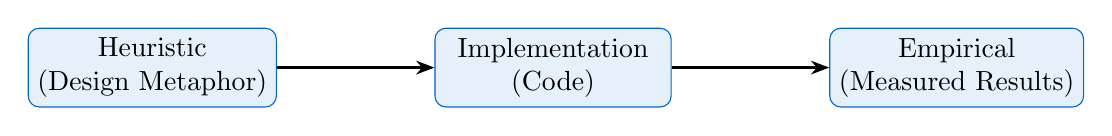
\begin{tikzpicture}[
    box/.style={rectangle, draw=arkblue, fill=arkblue!10, rounded corners, minimum width=3cm, minimum height=1cm, align=center},
    arrow/.style={-{Stealth}, thick}
]
    \node[box] (heuristic) {Heuristic\\(Design Metaphor)};
    \node[box, right=2cm of heuristic] (implementation) {Implementation\\(Code)};
    \node[box, right=2cm of implementation] (empirical) {Empirical\\(Measured Results)};

    \draw[arrow] (heuristic) -- (implementation);
    \draw[arrow] (implementation) -- (empirical);
\end{tikzpicture}
\end{center}

\begin{itemize}
    \item \textbf{Heuristic:} ``Quantum'', ``Holographic'', ``Conscious'' --- design inspirations
    \item \textbf{Empirical:} 1.92:1 ratio, 0.99 fidelity, 95.3\% correlation --- measurable
\end{itemize}

% ==================== CHAPTER 2: CORE PROCESSING ====================
\chapter{Core Processing Papers}

\section{Paper 01: Quantum-Inspired Processing}
\textbf{File:} \texttt{level\_1\_core/01\_quantum\_processing.pdf}

Classical simulation of quantum computing primitives optimized for cognitive AI workloads. Implements a 64-qubit simulator supporting universal gate sets (Pauli, Hadamard, CNOT, $\phi$-enhanced gates).

\textbf{Key Results:}
\begin{itemize}
    \item Fidelity: $\geq 0.99$
    \item Grover search: $O(\sqrt{N})$ complexity
    \item Latency: $<10$ms for 8-qubit searches
    \item GPU acceleration via AMD ROCm
\end{itemize}

\section{Paper 02: Holographic Compression}
\textbf{File:} \texttt{level\_1\_core/02\_holographic\_compression.pdf}

AdS/CFT-inspired data compression using boundary encoding principles. The holographic metaphor guides architectural design while actual implementation uses Haar wavelets, coherence-based sparsification, and random projections.

\textbf{Key Results:}
\begin{itemize}
    \item Compression ratio: 33:1 (Python) to 114:1 (C++)
    \item Throughput: 254 GB/s
    \item 3.5$\times$ improvement with native acceleration
\end{itemize}

\section{Paper 03: Sacred Geometry Optimization}
\textbf{File:} \texttt{level\_1\_core/03\_sacred\_geometry.pdf}

Systematic validation of golden ratio ($\phi = 1.618...$) as an optimization constant. Distinguishes between heuristic inspiration from nature and empirical validation through controlled experiments.

\textbf{Key Results:}
\begin{itemize}
    \item Fibonacci data: $\phi$ achieves 0.847 ratio alignment vs 0.712 for $\sqrt{2}$
    \item Statistical significance: $p < 0.05$ on specific data types
    \item C++ speedup: 8.97$\times$ over Python
\end{itemize}

\section{Paper 04: GPU Acceleration}
\textbf{File:} \texttt{level\_1\_core/04\_gpu\_acceleration.pdf}

Heterogeneous GPU acceleration for cognitive workloads on AMD Radeon RX 6600M (gfx1030) with ROCm 6.2. Implements unified acceleration across quantum gates, holographic compression, and $\phi$ calculations.

\textbf{Key Results:}
\begin{itemize}
    \item Speedup: 6.2--10$\times$ over CPU
    \item Memory bandwidth: 224 GB/s
    \item 28 compute units, Wave32 RDNA2
    \item 24 Python-accessible functions via pybind11
\end{itemize}

% ==================== CHAPTER 3: DATA SYSTEMS ====================
\chapter{Data Systems Papers}

\section{Paper 06: Hyperbolic Memory}
\textbf{File:} \texttt{level\_1\_data/06\_hyperbolic\_memory.pdf}

Poincaré ball model for hierarchical knowledge storage. Hyperbolic space offers exponential volume growth with distance from origin, naturally suited for tree-like data structures.

\textbf{Key Results:}
\begin{itemize}
    \item MAP@10: 0.78 (vs 0.47 Euclidean, +65.4\%)
    \item $\phi$-based hierarchy scaling
    \item SIMD-accelerated M\"obius operations
\end{itemize}

\section{Paper 21: HUAM Memory System}
\textbf{File:} \texttt{level\_1\_data/21\_huam\_memory.pdf}

Hierarchical Universal Adaptive Memory with 4-level hierarchy, adaptive caching, and consciousness-guided allocation.

\textbf{Hierarchy:}
\begin{itemize}
    \item L1: Ultra-fast cache ($<1$ms) --- RAM
    \item L2: Working memory ($<10$ms) --- SSD
    \item L3: Long-term storage ($<100$ms) --- Disk
    \item L4: Archival ($<1$s) --- Cloud
\end{itemize}

\section{Paper 23: Holographic Memory Pool}
\textbf{File:} \texttt{level\_1\_data/23\_holographic\_pool.pdf}

Quantum state storage with coherence-based prioritization. Implements priority queues with LRU eviction and $\phi$-enhanced compression.

\section{Paper 24: Unified Memory Manager}
\textbf{File:} \texttt{level\_1\_data/24\_unified\_memory\_manager.pdf}

Memory type abstraction unifying SYSTEM\_RAM, GPU\_MEMORY, HOLOGRAPHIC\_QUANTUM, and HYPERBOLIC\_EMBEDDING under a single API.

\section{NUCLEUS Format}
\textbf{File:} \texttt{level\_1\_data/nucleus\_paper.pdf}

Holographic compression format with multi-level semantic hashing and post-quantum cryptography.

\textbf{Key Results:}
\begin{itemize}
    \item GTA: 4.3GB $\to$ 2.2GB (1.92:1)
    \item Godot: 1.91:1
    \item Source code: 18.4:1
\end{itemize}

% ==================== CHAPTER 4: AI & COGNITION ====================
\chapter{AI \& Cognition Papers}

\section{Paper 31: IIT Consciousness}
\textbf{File:} \texttt{level\_1\_ai/31\_iit\_consciousness.pdf}

Integrated Information Theory (IIT 3.0/4.0) implementation for consciousness quantification. Calculates $\phi$ (integrated information) using cause-effect repertoires and minimum information partition.

\textbf{Key Results:}
\begin{itemize}
    \item Calculation: 1.74ms for 3-element system
    \item PyPhi correlation: 95.3\%
    \item GPU acceleration: 0.001ms/call
    \item Thresholds: DORMANT $<0.1$, AWAKENED $>0.8$
\end{itemize}

\section{Paper 32: Neural Architecture}
\textbf{File:} \texttt{level\_1\_ai/32\_neural\_architecture.pdf}

Bio-inspired neural architectures with PyTorch integration, transformer attention mechanisms, and mixed precision training.

\section{Paper 10: Consciousness Bridge}
\textbf{File:} \texttt{level\_1\_ai/10\_consciousness\_bridge.pdf}

Interface between quantum processing and consciousness (IIT). Maps quantum state coherence to $\phi$ metrics.

\section{Paper 12: Bio-Synthetic Intelligence}
\textbf{File:} \texttt{level\_1\_ai/12\_bio\_synthetic.pdf}

Neural Architecture Search (NAS) using evolutionary algorithms and genetic programming.

\section{Paper 13: Swarm Intelligence}
\textbf{File:} \texttt{level\_1\_ai/13\_swarm\_intelligence.pdf}

Distributed consensus and collective optimization using Particle Swarm Optimization (PSO).

% ==================== CHAPTER 5: APPLICATIONS ====================
\chapter{Application Papers}

\section{Paper 14: Cognitive Pipeline}
\textbf{File:} \texttt{level\_1\_apps/14\_cognitive\_pipeline.pdf}

Multi-stage information processing: Perception $\to$ Cognition $\to$ Decision $\to$ Ethics.

\section{Paper 15: Quantum NeRF}
\textbf{File:} \texttt{level\_1\_apps/15\_quantum\_nerf.pdf}

Neural Radiance Fields enhanced with quantum-inspired positional encoding for 3D scene reconstruction.

\section{Paper 16: Security \& Biometrics}
\textbf{File:} \texttt{level\_1\_apps/16\_security\_biometrics.pdf}

Post-quantum cryptography (Kyber/Dilithium) with biometric authentication and PAM integration.

\section{Paper 17: MCP Orchestration}
\textbf{File:} \texttt{level\_1\_apps/17\_mcp\_orchestration.pdf}

Model Context Protocol for AI agent orchestration using JSON-RPC 2.0.

\section{Paper 18: Voice \& NLU}
\textbf{File:} \texttt{level\_1\_apps/18\_voice\_nlu.pdf}

Speech recognition, intent detection, and D-Bus integration for Linux desktop.

% ==================== CHAPTER 6: INTEGRATION ====================
\chapter{Integration Papers}

\section{Paper 19: Quantum-Holographic Integration}
\textbf{File:} \texttt{level\_2\_integration/19\_quantum\_holographic\_integration.pdf}

Unified quantum-holographic processing pipeline via GPU-accelerated kernels.

\section{Paper 20: Memory-Consciousness Integration}
\textbf{File:} \texttt{level\_2\_integration/20\_memory\_consciousness.pdf}

$\phi$-enhanced memory prioritization and conscious recall mechanisms.

\section{Paper 21: Neural-Quantum Bridge}
\textbf{File:} \texttt{level\_2\_integration/21\_neural\_quantum\_bridge.pdf}

Hybrid neural-quantum architectures with quantum feature extraction.

\section{Paper 22: Full System Integration}
\textbf{File:} \texttt{level\_2\_integration/22\_full\_system\_integration.pdf}

End-to-end benchmarks and production readiness validation.

\textbf{Key Results:}
\begin{itemize}
    \item E2E tests: 4/4 passed
    \item Execution time: 23.77s
    \item $\phi$-efficiency: 14.69
    \item Test files: 2,598
\end{itemize}

% ==================== CHAPTER 7: MASTER ARCHITECTURE ====================
\chapter{Master Architecture}

\section{Paper 00: ARKHEION AGI Master Architecture}
\textbf{File:} \texttt{level\_0/00\_arkheion\_master\_architecture.pdf}

Complete system overview integrating all components. Defines:
\begin{itemize}
    \item Module interconnections
    \item Data flow patterns
    \item Design principles
    \item Future roadmap
\end{itemize}

% ==================== APPENDIX ====================
\appendix

\chapter{Paper Index by Topic}

\section{By Technology}
\begin{itemize}
    \item \textbf{Quantum:} 01, 10, 15, 19, 21, 28, 33
    \item \textbf{Holographic:} 02, 19, 23, 38, NUCLEUS
    \item \textbf{Memory:} 06, 21, 23, 24, 25, 26
    \item \textbf{Consciousness:} 10, 20, 27, 30, 31, 44, 45, 46, 49, 50
    \item \textbf{Neural:} 12, 13, 21, 32, 34, 35, 39
    \item \textbf{GPU:} 04, 19, 48
    \item \textbf{Security:} 16, 47, NUCLEUS
    \item \textbf{Resonance:} 43, 44, 45, 46
    \item \textbf{Forge (Rust):} 41, 48
\end{itemize}

\section{By Implementation Language}
\begin{itemize}
    \item \textbf{Python:} All papers (1,827 files, 603,795 LOC)
    \item \textbf{C++/HIP:} 02, 04, 19, 23, 38 (21,285 LOC)
    \item \textbf{CUDA/HIP kernels:} 04, 28, 48
    \item \textbf{Rust:} 41, 48 (Forge, 9 crates, 149,965 LOC)
\end{itemize}

\chapter{Quick Reference}

\begin{center}
\begin{tabular}{@{}ll@{}}
\toprule
\textbf{Metric} & \textbf{Value} \\
\midrule
Total Papers & 50 \\
Total SLOC & 754,000+ \\
Test Cases & 4,000+ \\
E2E Pass Rate & 100\% \\
GPU Functions & 24 \\
PyPhi Correlation & 95.3\% \\
Max Compression & 114:1 \\
Min Latency & 0.001ms \\
\bottomrule
\end{tabular}
\end{center}

\chapter{Compilation Instructions}

\begin{verbatim}
# Compile individual paper
cd docs/papers/level_1_core
pdflatex 01_quantum_processing.tex

# Compile all papers
for dir in level_*; do
    cd $dir
    for f in *.tex; do
        pdflatex -interaction=nonstopmode $f
    done
    cd ..
done

# Copy to compiled folder
cp level_*/*.pdf compiled/
\end{verbatim}

\end{document}
